\documentclass[twoside]{book}

% Packages required by doxygen
\usepackage{calc}
\usepackage{doxygen}
\usepackage{graphicx}
\usepackage[utf8]{inputenc}
\usepackage{makeidx}
\usepackage{multicol}
\usepackage{multirow}
\usepackage{textcomp}
\usepackage[table]{xcolor}

% Font selection
\usepackage[T1]{fontenc}
\usepackage{mathptmx}
\usepackage[scaled=.90]{helvet}
\usepackage{courier}
\usepackage{amssymb}
\usepackage{sectsty}
\renewcommand{\familydefault}{\sfdefault}
\allsectionsfont{%
  \fontseries{bc}\selectfont%
  \color{darkgray}%
}
\renewcommand{\DoxyLabelFont}{%
  \fontseries{bc}\selectfont%
  \color{darkgray}%
}

% Page & text layout
\usepackage{geometry}
\geometry{%
  a4paper,%
  top=2.5cm,%
  bottom=2.5cm,%
  left=2.5cm,%
  right=2.5cm%
}
\tolerance=750
\hfuzz=15pt
\hbadness=750
\setlength{\emergencystretch}{15pt}
\setlength{\parindent}{0cm}
\setlength{\parskip}{0.2cm}
\makeatletter
\renewcommand{\paragraph}{%
  \@startsection{paragraph}{4}{0ex}{-1.0ex}{1.0ex}{%
    \normalfont\normalsize\bfseries\SS@parafont%
  }%
}
\renewcommand{\subparagraph}{%
  \@startsection{subparagraph}{5}{0ex}{-1.0ex}{1.0ex}{%
    \normalfont\normalsize\bfseries\SS@subparafont%
  }%
}
\makeatother

% Headers & footers
\usepackage{fancyhdr}
\pagestyle{fancyplain}
\fancyhead[LE]{\fancyplain{}{\bfseries\thepage}}
\fancyhead[CE]{\fancyplain{}{}}
\fancyhead[RE]{\fancyplain{}{\bfseries\leftmark}}
\fancyhead[LO]{\fancyplain{}{\bfseries\rightmark}}
\fancyhead[CO]{\fancyplain{}{}}
\fancyhead[RO]{\fancyplain{}{\bfseries\thepage}}
\fancyfoot[LE]{\fancyplain{}{}}
\fancyfoot[CE]{\fancyplain{}{}}
\fancyfoot[RE]{\fancyplain{}{\bfseries\scriptsize Generated on Mon Jan 6 2014 03\-:58\-:16 for Zero\-Sync by Doxygen }}
\fancyfoot[LO]{\fancyplain{}{\bfseries\scriptsize Generated on Mon Jan 6 2014 03\-:58\-:16 for Zero\-Sync by Doxygen }}
\fancyfoot[CO]{\fancyplain{}{}}
\fancyfoot[RO]{\fancyplain{}{}}
\renewcommand{\footrulewidth}{0.4pt}
\renewcommand{\chaptermark}[1]{%
  \markboth{#1}{}%
}
\renewcommand{\sectionmark}[1]{%
  \markright{\thesection\ #1}%
}

% Indices & bibliography
\usepackage{natbib}
\usepackage[titles]{tocloft}
\setcounter{tocdepth}{3}
\setcounter{secnumdepth}{5}
\makeindex

% Hyperlinks (required, but should be loaded last)
\usepackage{ifpdf}
\ifpdf
  \usepackage[pdftex,pagebackref=true]{hyperref}
\else
  \usepackage[ps2pdf,pagebackref=true]{hyperref}
\fi
\hypersetup{%
  colorlinks=true,%
  linkcolor=blue,%
  citecolor=blue,%
  unicode%
}

% Custom commands
\newcommand{\clearemptydoublepage}{%
  \newpage{\pagestyle{empty}\cleardoublepage}%
}


%===== C O N T E N T S =====

\begin{document}

% Titlepage & ToC
\hypersetup{pageanchor=false}
\pagenumbering{roman}
\begin{titlepage}
\vspace*{7cm}
\begin{center}%
{\Large Zero\-Sync }\\
\vspace*{1cm}
{\large Generated by Doxygen 1.8.6}\\
\vspace*{0.5cm}
{\small Mon Jan 6 2014 03:58:16}\\
\end{center}
\end{titlepage}
\clearemptydoublepage
\tableofcontents
\clearemptydoublepage
\pagenumbering{arabic}
\hypersetup{pageanchor=true}

%--- Begin generated contents ---
\chapter{Namespace Index}
\section{Namespace List}
Here is a list of all namespaces with brief descriptions\-:\begin{DoxyCompactList}
\item\contentsline{section}{\hyperlink{namespace_ui}{Ui} }{\pageref{namespace_ui}}{}
\end{DoxyCompactList}

\chapter{Hierarchical Index}
\section{Class Hierarchy}
This inheritance list is sorted roughly, but not completely, alphabetically\-:\begin{DoxyCompactList}
\item Q\-Main\-Window\begin{DoxyCompactList}
\item \contentsline{section}{Main\-Window}{\pageref{class_main_window}}{}
\end{DoxyCompactList}
\item Q\-Object\begin{DoxyCompactList}
\item \contentsline{section}{Z\-S\-Database}{\pageref{class_z_s_database}}{}
\item \contentsline{section}{Z\-S\-File\-Meta\-Data}{\pageref{class_z_s_file_meta_data}}{}
\item \contentsline{section}{Z\-S\-File\-System\-Watcher}{\pageref{class_z_s_file_system_watcher}}{}
\item \contentsline{section}{Z\-S\-Index}{\pageref{class_z_s_index}}{}
\item \contentsline{section}{Z\-S\-Settings}{\pageref{class_z_s_settings}}{}
\item \contentsline{section}{Z\-S\-Setup\-Wizard}{\pageref{class_z_s_setup_wizard}}{}
\end{DoxyCompactList}
\end{DoxyCompactList}

\chapter{Class Index}
\section{Class List}
Here are the classes, structs, unions and interfaces with brief descriptions\-:\begin{DoxyCompactList}
\item\contentsline{section}{\hyperlink{class_main_window}{Main\-Window} }{\pageref{class_main_window}}{}
\item\contentsline{section}{\hyperlink{class_z_s_database}{Z\-S\-Database} }{\pageref{class_z_s_database}}{}
\item\contentsline{section}{\hyperlink{class_z_s_file_meta_data}{Z\-S\-File\-Meta\-Data} }{\pageref{class_z_s_file_meta_data}}{}
\item\contentsline{section}{\hyperlink{class_z_s_file_system_watcher}{Z\-S\-File\-System\-Watcher} }{\pageref{class_z_s_file_system_watcher}}{}
\item\contentsline{section}{\hyperlink{class_z_s_index}{Z\-S\-Index} }{\pageref{class_z_s_index}}{}
\item\contentsline{section}{\hyperlink{class_z_s_settings}{Z\-S\-Settings} }{\pageref{class_z_s_settings}}{}
\item\contentsline{section}{\hyperlink{class_z_s_setup_wizard}{Z\-S\-Setup\-Wizard} }{\pageref{class_z_s_setup_wizard}}{}
\end{DoxyCompactList}

\chapter{File Index}
\section{File List}
Here is a list of all files with brief descriptions\-:\begin{DoxyCompactList}
\item\contentsline{section}{C\-:/\-Users/adorno/github/zerodesk/\-Zero\-Sync\-Desktop/\hyperlink{main_8cpp}{main.\-cpp} }{\pageref{main_8cpp}}{}
\item\contentsline{section}{C\-:/\-Users/adorno/github/zerodesk/\-Zero\-Sync\-Desktop/\hyperlink{mainwindow_8cpp}{mainwindow.\-cpp} }{\pageref{mainwindow_8cpp}}{}
\item\contentsline{section}{C\-:/\-Users/adorno/github/zerodesk/\-Zero\-Sync\-Desktop/\hyperlink{mainwindow_8h}{mainwindow.\-h} }{\pageref{mainwindow_8h}}{}
\item\contentsline{section}{C\-:/\-Users/adorno/github/zerodesk/\-Zero\-Sync\-Desktop/\hyperlink{zsdatabase_8cpp}{zsdatabase.\-cpp} }{\pageref{zsdatabase_8cpp}}{}
\item\contentsline{section}{C\-:/\-Users/adorno/github/zerodesk/\-Zero\-Sync\-Desktop/\hyperlink{zsdatabase_8h}{zsdatabase.\-h} }{\pageref{zsdatabase_8h}}{}
\item\contentsline{section}{C\-:/\-Users/adorno/github/zerodesk/\-Zero\-Sync\-Desktop/\hyperlink{zsfilemetadata_8cpp}{zsfilemetadata.\-cpp} }{\pageref{zsfilemetadata_8cpp}}{}
\item\contentsline{section}{C\-:/\-Users/adorno/github/zerodesk/\-Zero\-Sync\-Desktop/\hyperlink{zsfilemetadata_8h}{zsfilemetadata.\-h} }{\pageref{zsfilemetadata_8h}}{}
\item\contentsline{section}{C\-:/\-Users/adorno/github/zerodesk/\-Zero\-Sync\-Desktop/\hyperlink{zsfilesystemwatcher_8cpp}{zsfilesystemwatcher.\-cpp} }{\pageref{zsfilesystemwatcher_8cpp}}{}
\item\contentsline{section}{C\-:/\-Users/adorno/github/zerodesk/\-Zero\-Sync\-Desktop/\hyperlink{zsfilesystemwatcher_8h}{zsfilesystemwatcher.\-h} }{\pageref{zsfilesystemwatcher_8h}}{}
\item\contentsline{section}{C\-:/\-Users/adorno/github/zerodesk/\-Zero\-Sync\-Desktop/\hyperlink{zsindex_8cpp}{zsindex.\-cpp} }{\pageref{zsindex_8cpp}}{}
\item\contentsline{section}{C\-:/\-Users/adorno/github/zerodesk/\-Zero\-Sync\-Desktop/\hyperlink{zsindex_8h}{zsindex.\-h} }{\pageref{zsindex_8h}}{}
\item\contentsline{section}{C\-:/\-Users/adorno/github/zerodesk/\-Zero\-Sync\-Desktop/\hyperlink{zssettings_8cpp}{zssettings.\-cpp} }{\pageref{zssettings_8cpp}}{}
\item\contentsline{section}{C\-:/\-Users/adorno/github/zerodesk/\-Zero\-Sync\-Desktop/\hyperlink{zssettings_8h}{zssettings.\-h} }{\pageref{zssettings_8h}}{}
\item\contentsline{section}{C\-:/\-Users/adorno/github/zerodesk/\-Zero\-Sync\-Desktop/\hyperlink{zssetupwizard_8cpp}{zssetupwizard.\-cpp} }{\pageref{zssetupwizard_8cpp}}{}
\item\contentsline{section}{C\-:/\-Users/adorno/github/zerodesk/\-Zero\-Sync\-Desktop/\hyperlink{zssetupwizard_8h}{zssetupwizard.\-h} }{\pageref{zssetupwizard_8h}}{}
\end{DoxyCompactList}

\chapter{Namespace Documentation}
\hypertarget{namespace_ui}{\section{Ui Namespace Reference}
\label{namespace_ui}\index{Ui@{Ui}}
}

\chapter{Class Documentation}
\hypertarget{class_main_window}{\section{Main\-Window Class Reference}
\label{class_main_window}\index{Main\-Window@{Main\-Window}}
}


{\ttfamily \#include $<$mainwindow.\-h$>$}

Inheritance diagram for Main\-Window\-:\begin{figure}[H]
\begin{center}
\leavevmode
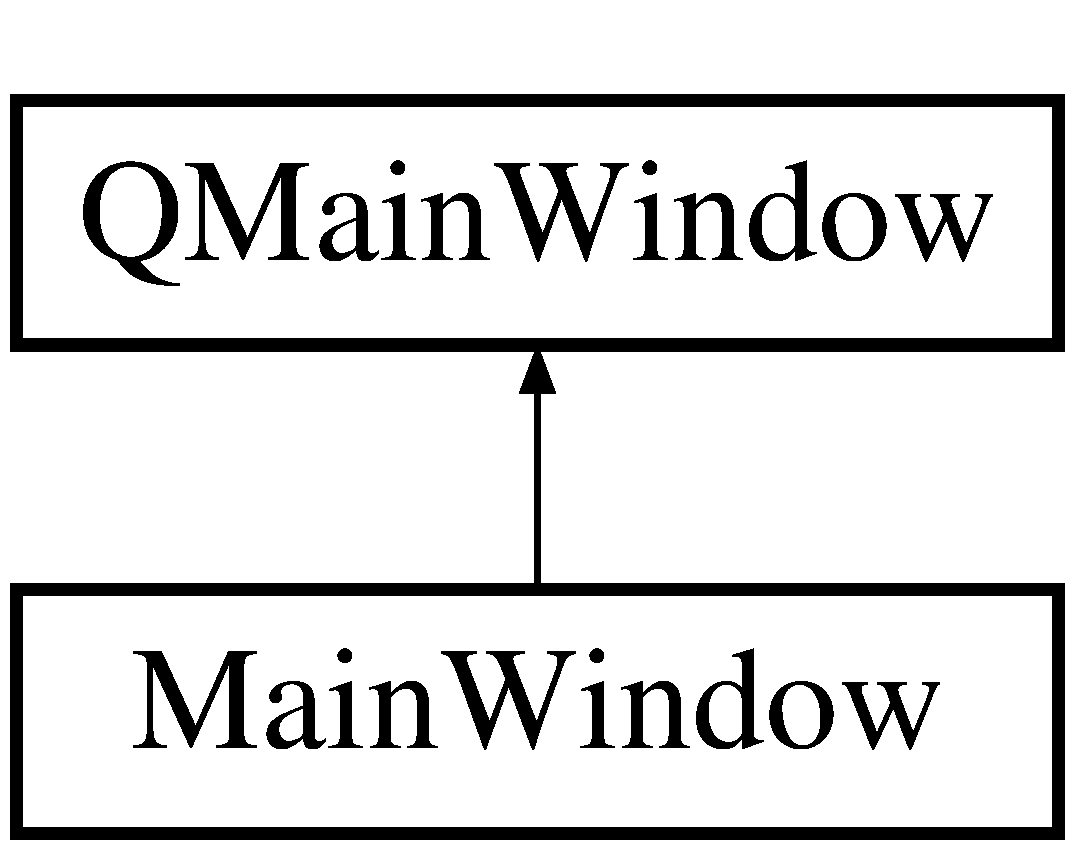
\includegraphics[height=2.000000cm]{class_main_window}
\end{center}
\end{figure}
\subsection*{Public Member Functions}
\begin{DoxyCompactItemize}
\item 
\hyperlink{class_main_window_a8b244be8b7b7db1b08de2a2acb9409db}{Main\-Window} (Q\-Widget $\ast$parent=0)
\item 
\hyperlink{class_main_window_ae98d00a93bc118200eeef9f9bba1dba7}{$\sim$\-Main\-Window} ()
\end{DoxyCompactItemize}


\subsection{Constructor \& Destructor Documentation}
\hypertarget{class_main_window_a8b244be8b7b7db1b08de2a2acb9409db}{\index{Main\-Window@{Main\-Window}!Main\-Window@{Main\-Window}}
\index{Main\-Window@{Main\-Window}!MainWindow@{Main\-Window}}
\subsubsection[{Main\-Window}]{\setlength{\rightskip}{0pt plus 5cm}Main\-Window\-::\-Main\-Window (
\begin{DoxyParamCaption}
\item[{Q\-Widget $\ast$}]{parent = {\ttfamily 0}}
\end{DoxyParamCaption}
)\hspace{0.3cm}{\ttfamily [explicit]}}}\label{class_main_window_a8b244be8b7b7db1b08de2a2acb9409db}
\hypertarget{class_main_window_ae98d00a93bc118200eeef9f9bba1dba7}{\index{Main\-Window@{Main\-Window}!$\sim$\-Main\-Window@{$\sim$\-Main\-Window}}
\index{$\sim$\-Main\-Window@{$\sim$\-Main\-Window}!MainWindow@{Main\-Window}}
\subsubsection[{$\sim$\-Main\-Window}]{\setlength{\rightskip}{0pt plus 5cm}Main\-Window\-::$\sim$\-Main\-Window (
\begin{DoxyParamCaption}
{}
\end{DoxyParamCaption}
)}}\label{class_main_window_ae98d00a93bc118200eeef9f9bba1dba7}


The documentation for this class was generated from the following files\-:\begin{DoxyCompactItemize}
\item 
C\-:/\-Users/adorno/github/zerodesk/\-Zero\-Sync\-Desktop/\hyperlink{mainwindow_8h}{mainwindow.\-h}\item 
C\-:/\-Users/adorno/github/zerodesk/\-Zero\-Sync\-Desktop/\hyperlink{mainwindow_8cpp}{mainwindow.\-cpp}\end{DoxyCompactItemize}

\hypertarget{class_z_s_database}{\section{Z\-S\-Database Class Reference}
\label{class_z_s_database}\index{Z\-S\-Database@{Z\-S\-Database}}
}


{\ttfamily \#include $<$zsdatabase.\-h$>$}

Inheritance diagram for Z\-S\-Database\-:\begin{figure}[H]
\begin{center}
\leavevmode
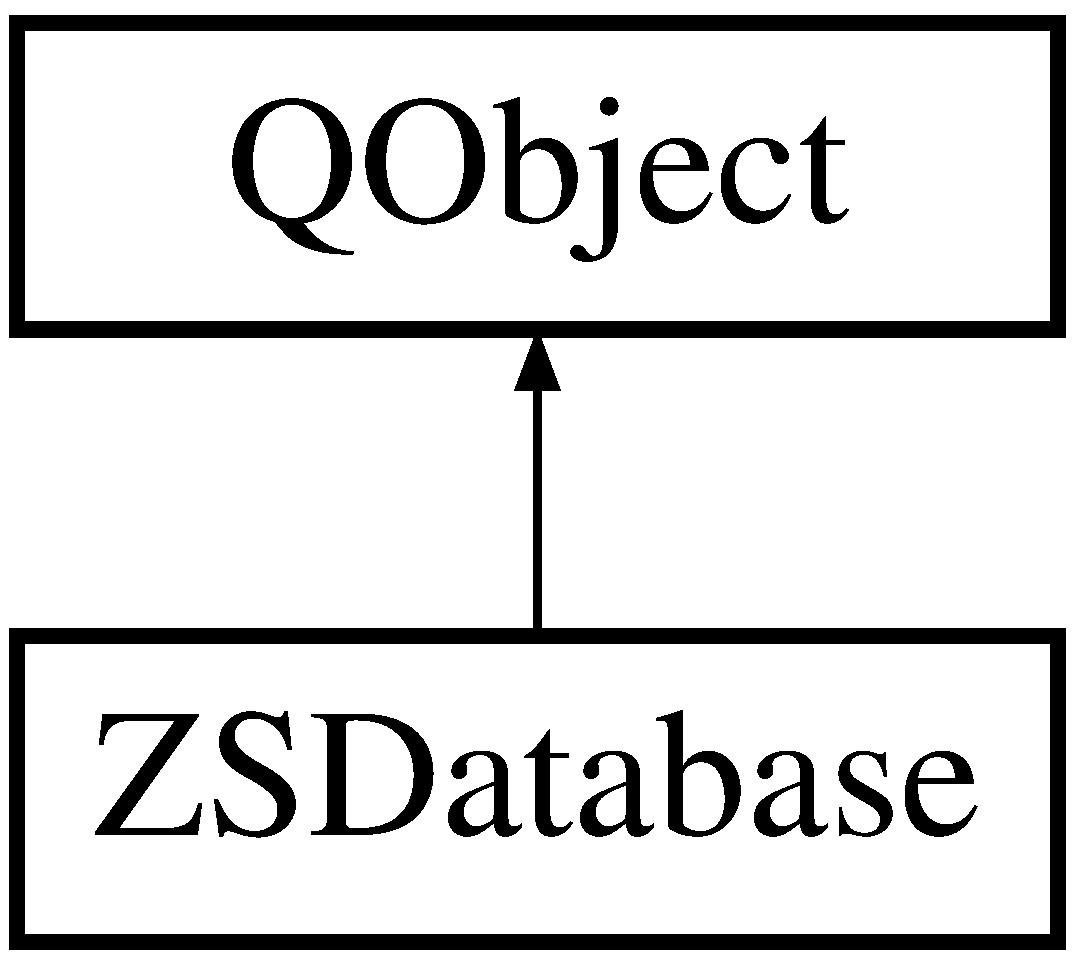
\includegraphics[height=2.000000cm]{class_z_s_database}
\end{center}
\end{figure}
\subsection*{Public Member Functions}
\begin{DoxyCompactItemize}
\item 
\hyperlink{class_z_s_database_a0627c12fe47bbde3e1170a5af8c184e6}{Z\-S\-Database} (Q\-Object $\ast$parent=0)
\item 
void \hyperlink{class_z_s_database_ac9bbe47e47751f4a414ff490eaa93f37}{insert\-New\-File} (Q\-String, qint64, Q\-String, qint64)
\item 
void \hyperlink{class_z_s_database_ad4a7a82f99dea6cae6eb2984e753e617}{set\-File\-Meta\-Data} (Q\-String, qint64, Q\-String, qint64)
\item 
void \hyperlink{class_z_s_database_abffe5b56804a6ab22c1000823b933457}{set\-File\-Changed} (Q\-String, int)
\item 
void \hyperlink{class_z_s_database_a5f7c4cec7800e5a988aa7655e5d6aba0}{set\-File\-Updated} (Q\-String, int)
\item 
void \hyperlink{class_z_s_database_a2bb1f63e20f29941aaa22d6d45706227}{set\-File\-Renamed} (Q\-String, int)
\item 
void \hyperlink{class_z_s_database_a5d64e9036561661bbfbcead13d80e732}{set\-File\-Deleted} (Q\-String, int)
\item 
void \hyperlink{class_z_s_database_ab48b210e0768ec84a14c495b375f54e9}{set\-New\-Path} (Q\-String, Q\-String)
\item 
Q\-String \hyperlink{class_z_s_database_ad2900311b21e3e04e993b4dcb86b59b3}{get\-File\-Path\-For\-Hash} (Q\-String)
\item 
void \hyperlink{class_z_s_database_a0bed2c815150aa6355872605d2e0fcf5}{set\-File\-Hash\-To\-Zero} (Q\-String)
\item 
bool \hyperlink{class_z_s_database_a065508a7f918f70b815b62ac46b84fc5}{is\-File\-Changed} (Q\-String)
\item 
bool \hyperlink{class_z_s_database_a8956c2e63f50eb34c2a4752111921064}{is\-File\-Updated} (Q\-String)
\item 
bool \hyperlink{class_z_s_database_a73a368af71d0fbed197072462ad22b6b}{is\-File\-Renamed} (Q\-String)
\item 
bool \hyperlink{class_z_s_database_a5a73cbe4cf20c29083b2dd23268fbdc1}{is\-File\-Deleted} (Q\-String)
\item 
bool \hyperlink{class_z_s_database_a9b70013e15474dcaa8eec3cb7eb1e37c}{exists\-File\-Entry} (Q\-String)
\item 
bool \hyperlink{class_z_s_database_ae9f9794a28f8ed60d591b0db9c9d89e8}{exists\-File\-Hash} (Q\-String)
\item 
Q\-Sql\-Query $\ast$ \hyperlink{class_z_s_database_a4bf120dd7f040333fe99e28b71c452d3}{fetch\-All\-Changed\-Entries} ()
\item 
void \hyperlink{class_z_s_database_a27fe7ff50698a23ae2b70441a9c25432}{insert\-New\-Index\-Entry} (int, Q\-String, Q\-String, qint64, qint64, Q\-String, Q\-String)
\item 
int \hyperlink{class_z_s_database_ae698d389bf2c46f387cbc12be7b5b551}{get\-Latest\-State} ()
\item 
void \hyperlink{class_z_s_database_ac07ffecec9eddf5e5593445f8ecd41fb}{reset\-File\-Meta\-Data} ()
\item 
void \hyperlink{class_z_s_database_a3851ff56ae60b4576f2b66372fdee493}{delete\-All\-Rows\-From\-Files\-Table} ()
\item 
void \hyperlink{class_z_s_database_aa0f3a42f066417112034188239be3d46}{set\-Zero\-Sync\-Folder\-Changed\-Flag\-To\-File\-Index\-Table} ()
\end{DoxyCompactItemize}


\subsection{Constructor \& Destructor Documentation}
\hypertarget{class_z_s_database_a0627c12fe47bbde3e1170a5af8c184e6}{\index{Z\-S\-Database@{Z\-S\-Database}!Z\-S\-Database@{Z\-S\-Database}}
\index{Z\-S\-Database@{Z\-S\-Database}!ZSDatabase@{Z\-S\-Database}}
\subsubsection[{Z\-S\-Database}]{\setlength{\rightskip}{0pt plus 5cm}Z\-S\-Database\-::\-Z\-S\-Database (
\begin{DoxyParamCaption}
\item[{Q\-Object $\ast$}]{parent = {\ttfamily 0}}
\end{DoxyParamCaption}
)\hspace{0.3cm}{\ttfamily [explicit]}}}\label{class_z_s_database_a0627c12fe47bbde3e1170a5af8c184e6}


\subsection{Member Function Documentation}
\hypertarget{class_z_s_database_a3851ff56ae60b4576f2b66372fdee493}{\index{Z\-S\-Database@{Z\-S\-Database}!delete\-All\-Rows\-From\-Files\-Table@{delete\-All\-Rows\-From\-Files\-Table}}
\index{delete\-All\-Rows\-From\-Files\-Table@{delete\-All\-Rows\-From\-Files\-Table}!ZSDatabase@{Z\-S\-Database}}
\subsubsection[{delete\-All\-Rows\-From\-Files\-Table}]{\setlength{\rightskip}{0pt plus 5cm}void Z\-S\-Database\-::delete\-All\-Rows\-From\-Files\-Table (
\begin{DoxyParamCaption}
{}
\end{DoxyParamCaption}
)}}\label{class_z_s_database_a3851ff56ae60b4576f2b66372fdee493}
\hypertarget{class_z_s_database_a9b70013e15474dcaa8eec3cb7eb1e37c}{\index{Z\-S\-Database@{Z\-S\-Database}!exists\-File\-Entry@{exists\-File\-Entry}}
\index{exists\-File\-Entry@{exists\-File\-Entry}!ZSDatabase@{Z\-S\-Database}}
\subsubsection[{exists\-File\-Entry}]{\setlength{\rightskip}{0pt plus 5cm}bool Z\-S\-Database\-::exists\-File\-Entry (
\begin{DoxyParamCaption}
\item[{Q\-String}]{path}
\end{DoxyParamCaption}
)}}\label{class_z_s_database_a9b70013e15474dcaa8eec3cb7eb1e37c}
\hypertarget{class_z_s_database_ae9f9794a28f8ed60d591b0db9c9d89e8}{\index{Z\-S\-Database@{Z\-S\-Database}!exists\-File\-Hash@{exists\-File\-Hash}}
\index{exists\-File\-Hash@{exists\-File\-Hash}!ZSDatabase@{Z\-S\-Database}}
\subsubsection[{exists\-File\-Hash}]{\setlength{\rightskip}{0pt plus 5cm}bool Z\-S\-Database\-::exists\-File\-Hash (
\begin{DoxyParamCaption}
\item[{Q\-String}]{checksum}
\end{DoxyParamCaption}
)}}\label{class_z_s_database_ae9f9794a28f8ed60d591b0db9c9d89e8}
\hypertarget{class_z_s_database_a4bf120dd7f040333fe99e28b71c452d3}{\index{Z\-S\-Database@{Z\-S\-Database}!fetch\-All\-Changed\-Entries@{fetch\-All\-Changed\-Entries}}
\index{fetch\-All\-Changed\-Entries@{fetch\-All\-Changed\-Entries}!ZSDatabase@{Z\-S\-Database}}
\subsubsection[{fetch\-All\-Changed\-Entries}]{\setlength{\rightskip}{0pt plus 5cm}Q\-Sql\-Query $\ast$ Z\-S\-Database\-::fetch\-All\-Changed\-Entries (
\begin{DoxyParamCaption}
{}
\end{DoxyParamCaption}
)}}\label{class_z_s_database_a4bf120dd7f040333fe99e28b71c452d3}
\hypertarget{class_z_s_database_ad2900311b21e3e04e993b4dcb86b59b3}{\index{Z\-S\-Database@{Z\-S\-Database}!get\-File\-Path\-For\-Hash@{get\-File\-Path\-For\-Hash}}
\index{get\-File\-Path\-For\-Hash@{get\-File\-Path\-For\-Hash}!ZSDatabase@{Z\-S\-Database}}
\subsubsection[{get\-File\-Path\-For\-Hash}]{\setlength{\rightskip}{0pt plus 5cm}Q\-String Z\-S\-Database\-::get\-File\-Path\-For\-Hash (
\begin{DoxyParamCaption}
\item[{Q\-String}]{hash}
\end{DoxyParamCaption}
)}}\label{class_z_s_database_ad2900311b21e3e04e993b4dcb86b59b3}
\hypertarget{class_z_s_database_ae698d389bf2c46f387cbc12be7b5b551}{\index{Z\-S\-Database@{Z\-S\-Database}!get\-Latest\-State@{get\-Latest\-State}}
\index{get\-Latest\-State@{get\-Latest\-State}!ZSDatabase@{Z\-S\-Database}}
\subsubsection[{get\-Latest\-State}]{\setlength{\rightskip}{0pt plus 5cm}int Z\-S\-Database\-::get\-Latest\-State (
\begin{DoxyParamCaption}
{}
\end{DoxyParamCaption}
)}}\label{class_z_s_database_ae698d389bf2c46f387cbc12be7b5b551}
\hypertarget{class_z_s_database_ac9bbe47e47751f4a414ff490eaa93f37}{\index{Z\-S\-Database@{Z\-S\-Database}!insert\-New\-File@{insert\-New\-File}}
\index{insert\-New\-File@{insert\-New\-File}!ZSDatabase@{Z\-S\-Database}}
\subsubsection[{insert\-New\-File}]{\setlength{\rightskip}{0pt plus 5cm}void Z\-S\-Database\-::insert\-New\-File (
\begin{DoxyParamCaption}
\item[{Q\-String}]{path, }
\item[{qint64}]{timestamp, }
\item[{Q\-String}]{checksum, }
\item[{qint64}]{size}
\end{DoxyParamCaption}
)}}\label{class_z_s_database_ac9bbe47e47751f4a414ff490eaa93f37}
\hypertarget{class_z_s_database_a27fe7ff50698a23ae2b70441a9c25432}{\index{Z\-S\-Database@{Z\-S\-Database}!insert\-New\-Index\-Entry@{insert\-New\-Index\-Entry}}
\index{insert\-New\-Index\-Entry@{insert\-New\-Index\-Entry}!ZSDatabase@{Z\-S\-Database}}
\subsubsection[{insert\-New\-Index\-Entry}]{\setlength{\rightskip}{0pt plus 5cm}void Z\-S\-Database\-::insert\-New\-Index\-Entry (
\begin{DoxyParamCaption}
\item[{int}]{state, }
\item[{Q\-String}]{path, }
\item[{Q\-String}]{operation, }
\item[{qint64}]{timestamp, }
\item[{qint64}]{size, }
\item[{Q\-String}]{newpath, }
\item[{Q\-String}]{checksum}
\end{DoxyParamCaption}
)}}\label{class_z_s_database_a27fe7ff50698a23ae2b70441a9c25432}
\hypertarget{class_z_s_database_a065508a7f918f70b815b62ac46b84fc5}{\index{Z\-S\-Database@{Z\-S\-Database}!is\-File\-Changed@{is\-File\-Changed}}
\index{is\-File\-Changed@{is\-File\-Changed}!ZSDatabase@{Z\-S\-Database}}
\subsubsection[{is\-File\-Changed}]{\setlength{\rightskip}{0pt plus 5cm}bool Z\-S\-Database\-::is\-File\-Changed (
\begin{DoxyParamCaption}
\item[{Q\-String}]{path}
\end{DoxyParamCaption}
)}}\label{class_z_s_database_a065508a7f918f70b815b62ac46b84fc5}
\hypertarget{class_z_s_database_a5a73cbe4cf20c29083b2dd23268fbdc1}{\index{Z\-S\-Database@{Z\-S\-Database}!is\-File\-Deleted@{is\-File\-Deleted}}
\index{is\-File\-Deleted@{is\-File\-Deleted}!ZSDatabase@{Z\-S\-Database}}
\subsubsection[{is\-File\-Deleted}]{\setlength{\rightskip}{0pt plus 5cm}bool Z\-S\-Database\-::is\-File\-Deleted (
\begin{DoxyParamCaption}
\item[{Q\-String}]{path}
\end{DoxyParamCaption}
)}}\label{class_z_s_database_a5a73cbe4cf20c29083b2dd23268fbdc1}
\hypertarget{class_z_s_database_a73a368af71d0fbed197072462ad22b6b}{\index{Z\-S\-Database@{Z\-S\-Database}!is\-File\-Renamed@{is\-File\-Renamed}}
\index{is\-File\-Renamed@{is\-File\-Renamed}!ZSDatabase@{Z\-S\-Database}}
\subsubsection[{is\-File\-Renamed}]{\setlength{\rightskip}{0pt plus 5cm}bool Z\-S\-Database\-::is\-File\-Renamed (
\begin{DoxyParamCaption}
\item[{Q\-String}]{path}
\end{DoxyParamCaption}
)}}\label{class_z_s_database_a73a368af71d0fbed197072462ad22b6b}
\hypertarget{class_z_s_database_a8956c2e63f50eb34c2a4752111921064}{\index{Z\-S\-Database@{Z\-S\-Database}!is\-File\-Updated@{is\-File\-Updated}}
\index{is\-File\-Updated@{is\-File\-Updated}!ZSDatabase@{Z\-S\-Database}}
\subsubsection[{is\-File\-Updated}]{\setlength{\rightskip}{0pt plus 5cm}bool Z\-S\-Database\-::is\-File\-Updated (
\begin{DoxyParamCaption}
\item[{Q\-String}]{path}
\end{DoxyParamCaption}
)}}\label{class_z_s_database_a8956c2e63f50eb34c2a4752111921064}
\hypertarget{class_z_s_database_ac07ffecec9eddf5e5593445f8ecd41fb}{\index{Z\-S\-Database@{Z\-S\-Database}!reset\-File\-Meta\-Data@{reset\-File\-Meta\-Data}}
\index{reset\-File\-Meta\-Data@{reset\-File\-Meta\-Data}!ZSDatabase@{Z\-S\-Database}}
\subsubsection[{reset\-File\-Meta\-Data}]{\setlength{\rightskip}{0pt plus 5cm}void Z\-S\-Database\-::reset\-File\-Meta\-Data (
\begin{DoxyParamCaption}
{}
\end{DoxyParamCaption}
)}}\label{class_z_s_database_ac07ffecec9eddf5e5593445f8ecd41fb}
\hypertarget{class_z_s_database_abffe5b56804a6ab22c1000823b933457}{\index{Z\-S\-Database@{Z\-S\-Database}!set\-File\-Changed@{set\-File\-Changed}}
\index{set\-File\-Changed@{set\-File\-Changed}!ZSDatabase@{Z\-S\-Database}}
\subsubsection[{set\-File\-Changed}]{\setlength{\rightskip}{0pt plus 5cm}void Z\-S\-Database\-::set\-File\-Changed (
\begin{DoxyParamCaption}
\item[{Q\-String}]{path, }
\item[{int}]{value}
\end{DoxyParamCaption}
)}}\label{class_z_s_database_abffe5b56804a6ab22c1000823b933457}
\hypertarget{class_z_s_database_a5d64e9036561661bbfbcead13d80e732}{\index{Z\-S\-Database@{Z\-S\-Database}!set\-File\-Deleted@{set\-File\-Deleted}}
\index{set\-File\-Deleted@{set\-File\-Deleted}!ZSDatabase@{Z\-S\-Database}}
\subsubsection[{set\-File\-Deleted}]{\setlength{\rightskip}{0pt plus 5cm}void Z\-S\-Database\-::set\-File\-Deleted (
\begin{DoxyParamCaption}
\item[{Q\-String}]{path, }
\item[{int}]{value}
\end{DoxyParamCaption}
)}}\label{class_z_s_database_a5d64e9036561661bbfbcead13d80e732}
\hypertarget{class_z_s_database_a0bed2c815150aa6355872605d2e0fcf5}{\index{Z\-S\-Database@{Z\-S\-Database}!set\-File\-Hash\-To\-Zero@{set\-File\-Hash\-To\-Zero}}
\index{set\-File\-Hash\-To\-Zero@{set\-File\-Hash\-To\-Zero}!ZSDatabase@{Z\-S\-Database}}
\subsubsection[{set\-File\-Hash\-To\-Zero}]{\setlength{\rightskip}{0pt plus 5cm}void Z\-S\-Database\-::set\-File\-Hash\-To\-Zero (
\begin{DoxyParamCaption}
\item[{Q\-String}]{path}
\end{DoxyParamCaption}
)}}\label{class_z_s_database_a0bed2c815150aa6355872605d2e0fcf5}
\hypertarget{class_z_s_database_ad4a7a82f99dea6cae6eb2984e753e617}{\index{Z\-S\-Database@{Z\-S\-Database}!set\-File\-Meta\-Data@{set\-File\-Meta\-Data}}
\index{set\-File\-Meta\-Data@{set\-File\-Meta\-Data}!ZSDatabase@{Z\-S\-Database}}
\subsubsection[{set\-File\-Meta\-Data}]{\setlength{\rightskip}{0pt plus 5cm}void Z\-S\-Database\-::set\-File\-Meta\-Data (
\begin{DoxyParamCaption}
\item[{Q\-String}]{path, }
\item[{qint64}]{timestamp, }
\item[{Q\-String}]{checksum, }
\item[{qint64}]{size}
\end{DoxyParamCaption}
)}}\label{class_z_s_database_ad4a7a82f99dea6cae6eb2984e753e617}
\hypertarget{class_z_s_database_a2bb1f63e20f29941aaa22d6d45706227}{\index{Z\-S\-Database@{Z\-S\-Database}!set\-File\-Renamed@{set\-File\-Renamed}}
\index{set\-File\-Renamed@{set\-File\-Renamed}!ZSDatabase@{Z\-S\-Database}}
\subsubsection[{set\-File\-Renamed}]{\setlength{\rightskip}{0pt plus 5cm}void Z\-S\-Database\-::set\-File\-Renamed (
\begin{DoxyParamCaption}
\item[{Q\-String}]{path, }
\item[{int}]{value}
\end{DoxyParamCaption}
)}}\label{class_z_s_database_a2bb1f63e20f29941aaa22d6d45706227}
\hypertarget{class_z_s_database_a5f7c4cec7800e5a988aa7655e5d6aba0}{\index{Z\-S\-Database@{Z\-S\-Database}!set\-File\-Updated@{set\-File\-Updated}}
\index{set\-File\-Updated@{set\-File\-Updated}!ZSDatabase@{Z\-S\-Database}}
\subsubsection[{set\-File\-Updated}]{\setlength{\rightskip}{0pt plus 5cm}void Z\-S\-Database\-::set\-File\-Updated (
\begin{DoxyParamCaption}
\item[{Q\-String}]{path, }
\item[{int}]{value}
\end{DoxyParamCaption}
)}}\label{class_z_s_database_a5f7c4cec7800e5a988aa7655e5d6aba0}
\hypertarget{class_z_s_database_ab48b210e0768ec84a14c495b375f54e9}{\index{Z\-S\-Database@{Z\-S\-Database}!set\-New\-Path@{set\-New\-Path}}
\index{set\-New\-Path@{set\-New\-Path}!ZSDatabase@{Z\-S\-Database}}
\subsubsection[{set\-New\-Path}]{\setlength{\rightskip}{0pt plus 5cm}void Z\-S\-Database\-::set\-New\-Path (
\begin{DoxyParamCaption}
\item[{Q\-String}]{path, }
\item[{Q\-String}]{new\-Path}
\end{DoxyParamCaption}
)}}\label{class_z_s_database_ab48b210e0768ec84a14c495b375f54e9}
\hypertarget{class_z_s_database_aa0f3a42f066417112034188239be3d46}{\index{Z\-S\-Database@{Z\-S\-Database}!set\-Zero\-Sync\-Folder\-Changed\-Flag\-To\-File\-Index\-Table@{set\-Zero\-Sync\-Folder\-Changed\-Flag\-To\-File\-Index\-Table}}
\index{set\-Zero\-Sync\-Folder\-Changed\-Flag\-To\-File\-Index\-Table@{set\-Zero\-Sync\-Folder\-Changed\-Flag\-To\-File\-Index\-Table}!ZSDatabase@{Z\-S\-Database}}
\subsubsection[{set\-Zero\-Sync\-Folder\-Changed\-Flag\-To\-File\-Index\-Table}]{\setlength{\rightskip}{0pt plus 5cm}void Z\-S\-Database\-::set\-Zero\-Sync\-Folder\-Changed\-Flag\-To\-File\-Index\-Table (
\begin{DoxyParamCaption}
{}
\end{DoxyParamCaption}
)}}\label{class_z_s_database_aa0f3a42f066417112034188239be3d46}


The documentation for this class was generated from the following files\-:\begin{DoxyCompactItemize}
\item 
C\-:/\-Users/\-Tommy/workspace/cpp/zerodesk/\-Zero\-Sync\-Desktop/\hyperlink{zsdatabase_8h}{zsdatabase.\-h}\item 
C\-:/\-Users/\-Tommy/workspace/cpp/zerodesk/\-Zero\-Sync\-Desktop/\hyperlink{zsdatabase_8cpp}{zsdatabase.\-cpp}\end{DoxyCompactItemize}

\input{class_z_s_directory_wizard_page}
\hypertarget{class_z_s_file_meta_data}{\section{Z\-S\-File\-Meta\-Data Class Reference}
\label{class_z_s_file_meta_data}\index{Z\-S\-File\-Meta\-Data@{Z\-S\-File\-Meta\-Data}}
}


{\ttfamily \#include $<$zsfilemetadata.\-h$>$}

Inheritance diagram for Z\-S\-File\-Meta\-Data\-:\begin{figure}[H]
\begin{center}
\leavevmode
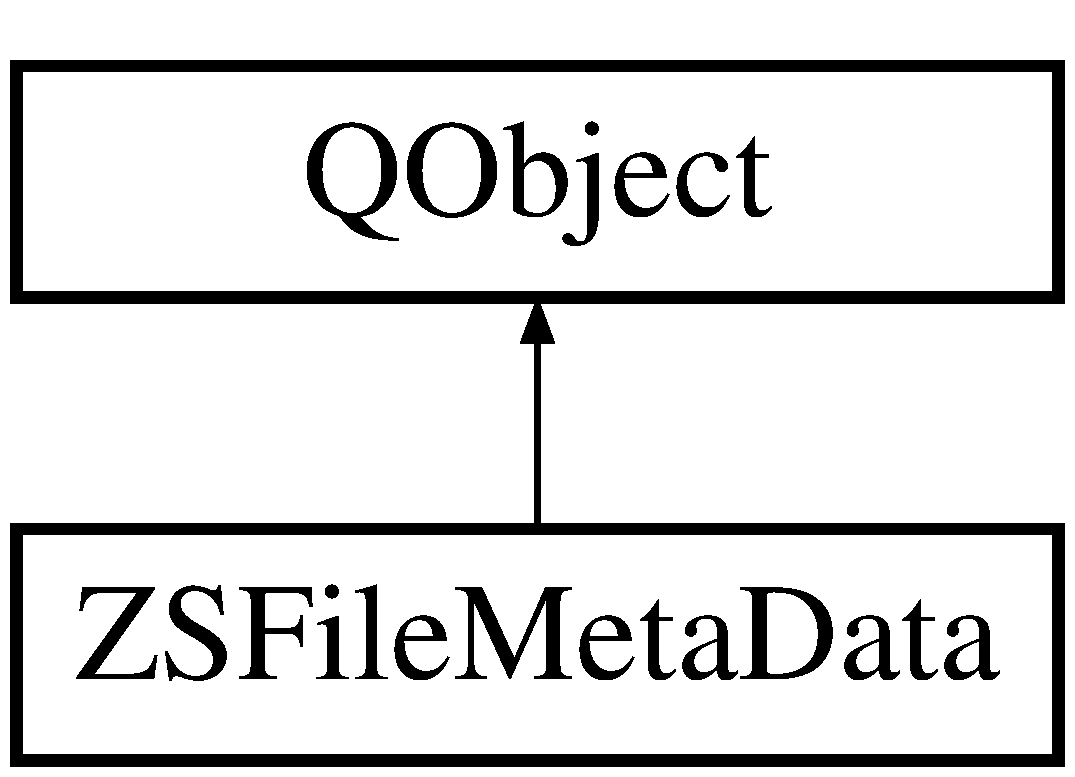
\includegraphics[height=2.000000cm]{class_z_s_file_meta_data}
\end{center}
\end{figure}
\subsection*{Public Member Functions}
\begin{DoxyCompactItemize}
\item 
\hyperlink{class_z_s_file_meta_data_a731a478cefcc8a9309d3a7c7c3a515f8}{Z\-S\-File\-Meta\-Data} (Q\-Object $\ast$parent=0, Q\-String path=Q\-String(), Q\-String path\-To\-Zero\-Sync\-Directory=Q\-String())
\item 
Q\-String \hyperlink{class_z_s_file_meta_data_a4de8705252b5f4f04d1327110f9fb97f}{get\-File\-Path} ()
\item 
qint64 \hyperlink{class_z_s_file_meta_data_a74c6702b8c5e79616ac6f1471f592e11}{get\-Last\-Modified} ()
\item 
Q\-String \hyperlink{class_z_s_file_meta_data_aa4330405660f5f326153b692b87477a2}{get\-Hash} ()
\item 
qint64 \hyperlink{class_z_s_file_meta_data_a7f3e513e794d08fb4e2d7c54b7b170be}{get\-File\-Size} ()
\end{DoxyCompactItemize}


\subsection{Constructor \& Destructor Documentation}
\hypertarget{class_z_s_file_meta_data_a731a478cefcc8a9309d3a7c7c3a515f8}{\index{Z\-S\-File\-Meta\-Data@{Z\-S\-File\-Meta\-Data}!Z\-S\-File\-Meta\-Data@{Z\-S\-File\-Meta\-Data}}
\index{Z\-S\-File\-Meta\-Data@{Z\-S\-File\-Meta\-Data}!ZSFileMetaData@{Z\-S\-File\-Meta\-Data}}
\subsubsection[{Z\-S\-File\-Meta\-Data}]{\setlength{\rightskip}{0pt plus 5cm}Z\-S\-File\-Meta\-Data\-::\-Z\-S\-File\-Meta\-Data (
\begin{DoxyParamCaption}
\item[{Q\-Object $\ast$}]{parent = {\ttfamily 0}, }
\item[{Q\-String}]{path = {\ttfamily QString()}, }
\item[{Q\-String}]{path\-To\-Zero\-Sync\-Directory = {\ttfamily QString()}}
\end{DoxyParamCaption}
)\hspace{0.3cm}{\ttfamily [explicit]}}}\label{class_z_s_file_meta_data_a731a478cefcc8a9309d3a7c7c3a515f8}


\subsection{Member Function Documentation}
\hypertarget{class_z_s_file_meta_data_a4de8705252b5f4f04d1327110f9fb97f}{\index{Z\-S\-File\-Meta\-Data@{Z\-S\-File\-Meta\-Data}!get\-File\-Path@{get\-File\-Path}}
\index{get\-File\-Path@{get\-File\-Path}!ZSFileMetaData@{Z\-S\-File\-Meta\-Data}}
\subsubsection[{get\-File\-Path}]{\setlength{\rightskip}{0pt plus 5cm}Q\-String Z\-S\-File\-Meta\-Data\-::get\-File\-Path (
\begin{DoxyParamCaption}
{}
\end{DoxyParamCaption}
)}}\label{class_z_s_file_meta_data_a4de8705252b5f4f04d1327110f9fb97f}
\hypertarget{class_z_s_file_meta_data_a7f3e513e794d08fb4e2d7c54b7b170be}{\index{Z\-S\-File\-Meta\-Data@{Z\-S\-File\-Meta\-Data}!get\-File\-Size@{get\-File\-Size}}
\index{get\-File\-Size@{get\-File\-Size}!ZSFileMetaData@{Z\-S\-File\-Meta\-Data}}
\subsubsection[{get\-File\-Size}]{\setlength{\rightskip}{0pt plus 5cm}qint64 Z\-S\-File\-Meta\-Data\-::get\-File\-Size (
\begin{DoxyParamCaption}
{}
\end{DoxyParamCaption}
)}}\label{class_z_s_file_meta_data_a7f3e513e794d08fb4e2d7c54b7b170be}
\hypertarget{class_z_s_file_meta_data_aa4330405660f5f326153b692b87477a2}{\index{Z\-S\-File\-Meta\-Data@{Z\-S\-File\-Meta\-Data}!get\-Hash@{get\-Hash}}
\index{get\-Hash@{get\-Hash}!ZSFileMetaData@{Z\-S\-File\-Meta\-Data}}
\subsubsection[{get\-Hash}]{\setlength{\rightskip}{0pt plus 5cm}Q\-String Z\-S\-File\-Meta\-Data\-::get\-Hash (
\begin{DoxyParamCaption}
{}
\end{DoxyParamCaption}
)}}\label{class_z_s_file_meta_data_aa4330405660f5f326153b692b87477a2}
\hypertarget{class_z_s_file_meta_data_a74c6702b8c5e79616ac6f1471f592e11}{\index{Z\-S\-File\-Meta\-Data@{Z\-S\-File\-Meta\-Data}!get\-Last\-Modified@{get\-Last\-Modified}}
\index{get\-Last\-Modified@{get\-Last\-Modified}!ZSFileMetaData@{Z\-S\-File\-Meta\-Data}}
\subsubsection[{get\-Last\-Modified}]{\setlength{\rightskip}{0pt plus 5cm}qint64 Z\-S\-File\-Meta\-Data\-::get\-Last\-Modified (
\begin{DoxyParamCaption}
{}
\end{DoxyParamCaption}
)}}\label{class_z_s_file_meta_data_a74c6702b8c5e79616ac6f1471f592e11}


The documentation for this class was generated from the following files\-:\begin{DoxyCompactItemize}
\item 
C\-:/\-Users/adorno/github/zerodesk/\-Zero\-Sync\-Desktop/\hyperlink{zsfilemetadata_8h}{zsfilemetadata.\-h}\item 
C\-:/\-Users/adorno/github/zerodesk/\-Zero\-Sync\-Desktop/\hyperlink{zsfilemetadata_8cpp}{zsfilemetadata.\-cpp}\end{DoxyCompactItemize}

\hypertarget{class_z_s_file_system_watcher}{\section{Z\-S\-File\-System\-Watcher Class Reference}
\label{class_z_s_file_system_watcher}\index{Z\-S\-File\-System\-Watcher@{Z\-S\-File\-System\-Watcher}}
}


{\ttfamily \#include $<$zsfilesystemwatcher.\-h$>$}

Inheritance diagram for Z\-S\-File\-System\-Watcher\-:\begin{figure}[H]
\begin{center}
\leavevmode
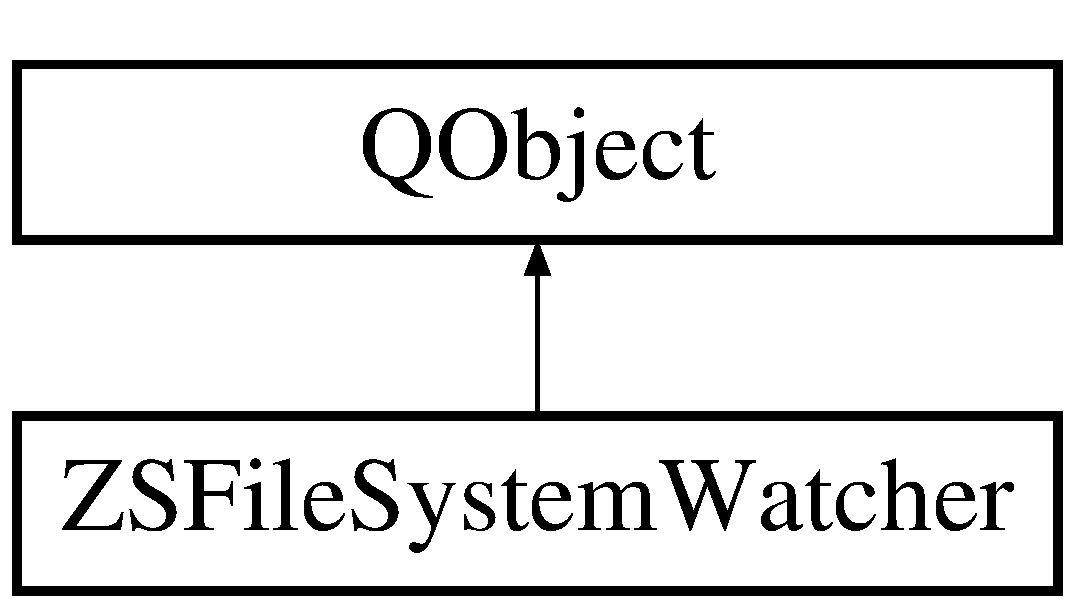
\includegraphics[height=2.000000cm]{class_z_s_file_system_watcher}
\end{center}
\end{figure}
\subsection*{Signals}
\begin{DoxyCompactItemize}
\item 
void \hyperlink{class_z_s_file_system_watcher_a480eedeb0d335cf692c002b710c3c94b}{signal\-Directory\-Change\-Recognized} (Q\-String)
\item 
void \hyperlink{class_z_s_file_system_watcher_a118b7f9b6356b07729ad2167921da4fd}{signal\-File\-Change\-Recognized} (Q\-String)
\end{DoxyCompactItemize}
\subsection*{Public Member Functions}
\begin{DoxyCompactItemize}
\item 
\hyperlink{class_z_s_file_system_watcher_a1d28ccc55263ad5af3155bad1048bf7d}{Z\-S\-File\-System\-Watcher} (Q\-Object $\ast$parent=0, \hyperlink{class_z_s_database}{Z\-S\-Database} $\ast$zsdatabase=0)
\item 
void \hyperlink{class_z_s_file_system_watcher_a99a18ceeab7e24dc79a7cd00003691c6}{set\-Zero\-Sync\-Directory} (Q\-String)
\item 
void \hyperlink{class_z_s_file_system_watcher_a4d4de58c5b1d09da7b15f7f25a82c60b}{change\-Zero\-Sync\-Directory} (Q\-String)
\end{DoxyCompactItemize}


\subsection{Constructor \& Destructor Documentation}
\hypertarget{class_z_s_file_system_watcher_a1d28ccc55263ad5af3155bad1048bf7d}{\index{Z\-S\-File\-System\-Watcher@{Z\-S\-File\-System\-Watcher}!Z\-S\-File\-System\-Watcher@{Z\-S\-File\-System\-Watcher}}
\index{Z\-S\-File\-System\-Watcher@{Z\-S\-File\-System\-Watcher}!ZSFileSystemWatcher@{Z\-S\-File\-System\-Watcher}}
\subsubsection[{Z\-S\-File\-System\-Watcher}]{\setlength{\rightskip}{0pt plus 5cm}Z\-S\-File\-System\-Watcher\-::\-Z\-S\-File\-System\-Watcher (
\begin{DoxyParamCaption}
\item[{Q\-Object $\ast$}]{parent = {\ttfamily 0}, }
\item[{{\bf Z\-S\-Database} $\ast$}]{zsdatabase = {\ttfamily 0}}
\end{DoxyParamCaption}
)\hspace{0.3cm}{\ttfamily [explicit]}}}\label{class_z_s_file_system_watcher_a1d28ccc55263ad5af3155bad1048bf7d}


\subsection{Member Function Documentation}
\hypertarget{class_z_s_file_system_watcher_a4d4de58c5b1d09da7b15f7f25a82c60b}{\index{Z\-S\-File\-System\-Watcher@{Z\-S\-File\-System\-Watcher}!change\-Zero\-Sync\-Directory@{change\-Zero\-Sync\-Directory}}
\index{change\-Zero\-Sync\-Directory@{change\-Zero\-Sync\-Directory}!ZSFileSystemWatcher@{Z\-S\-File\-System\-Watcher}}
\subsubsection[{change\-Zero\-Sync\-Directory}]{\setlength{\rightskip}{0pt plus 5cm}void Z\-S\-File\-System\-Watcher\-::change\-Zero\-Sync\-Directory (
\begin{DoxyParamCaption}
\item[{Q\-String}]{path\-To\-Directory}
\end{DoxyParamCaption}
)}}\label{class_z_s_file_system_watcher_a4d4de58c5b1d09da7b15f7f25a82c60b}
\hypertarget{class_z_s_file_system_watcher_a99a18ceeab7e24dc79a7cd00003691c6}{\index{Z\-S\-File\-System\-Watcher@{Z\-S\-File\-System\-Watcher}!set\-Zero\-Sync\-Directory@{set\-Zero\-Sync\-Directory}}
\index{set\-Zero\-Sync\-Directory@{set\-Zero\-Sync\-Directory}!ZSFileSystemWatcher@{Z\-S\-File\-System\-Watcher}}
\subsubsection[{set\-Zero\-Sync\-Directory}]{\setlength{\rightskip}{0pt plus 5cm}void Z\-S\-File\-System\-Watcher\-::set\-Zero\-Sync\-Directory (
\begin{DoxyParamCaption}
\item[{Q\-String}]{path\-To\-Directory}
\end{DoxyParamCaption}
)}}\label{class_z_s_file_system_watcher_a99a18ceeab7e24dc79a7cd00003691c6}
\hypertarget{class_z_s_file_system_watcher_a480eedeb0d335cf692c002b710c3c94b}{\index{Z\-S\-File\-System\-Watcher@{Z\-S\-File\-System\-Watcher}!signal\-Directory\-Change\-Recognized@{signal\-Directory\-Change\-Recognized}}
\index{signal\-Directory\-Change\-Recognized@{signal\-Directory\-Change\-Recognized}!ZSFileSystemWatcher@{Z\-S\-File\-System\-Watcher}}
\subsubsection[{signal\-Directory\-Change\-Recognized}]{\setlength{\rightskip}{0pt plus 5cm}void Z\-S\-File\-System\-Watcher\-::signal\-Directory\-Change\-Recognized (
\begin{DoxyParamCaption}
\item[{Q\-String}]{}
\end{DoxyParamCaption}
)\hspace{0.3cm}{\ttfamily [signal]}}}\label{class_z_s_file_system_watcher_a480eedeb0d335cf692c002b710c3c94b}
\hypertarget{class_z_s_file_system_watcher_a118b7f9b6356b07729ad2167921da4fd}{\index{Z\-S\-File\-System\-Watcher@{Z\-S\-File\-System\-Watcher}!signal\-File\-Change\-Recognized@{signal\-File\-Change\-Recognized}}
\index{signal\-File\-Change\-Recognized@{signal\-File\-Change\-Recognized}!ZSFileSystemWatcher@{Z\-S\-File\-System\-Watcher}}
\subsubsection[{signal\-File\-Change\-Recognized}]{\setlength{\rightskip}{0pt plus 5cm}void Z\-S\-File\-System\-Watcher\-::signal\-File\-Change\-Recognized (
\begin{DoxyParamCaption}
\item[{Q\-String}]{}
\end{DoxyParamCaption}
)\hspace{0.3cm}{\ttfamily [signal]}}}\label{class_z_s_file_system_watcher_a118b7f9b6356b07729ad2167921da4fd}


The documentation for this class was generated from the following files\-:\begin{DoxyCompactItemize}
\item 
C\-:/\-Users/\-Tommy/workspace/cpp/zerodesk/\-Zero\-Sync\-Desktop/\hyperlink{zsfilesystemwatcher_8h}{zsfilesystemwatcher.\-h}\item 
C\-:/\-Users/\-Tommy/workspace/cpp/zerodesk/\-Zero\-Sync\-Desktop/\hyperlink{zsfilesystemwatcher_8cpp}{zsfilesystemwatcher.\-cpp}\end{DoxyCompactItemize}

\hypertarget{class_z_s_index}{\section{Z\-S\-Index Class Reference}
\label{class_z_s_index}\index{Z\-S\-Index@{Z\-S\-Index}}
}


{\ttfamily \#include $<$zsindex.\-h$>$}

Inheritance diagram for Z\-S\-Index\-:\begin{figure}[H]
\begin{center}
\leavevmode
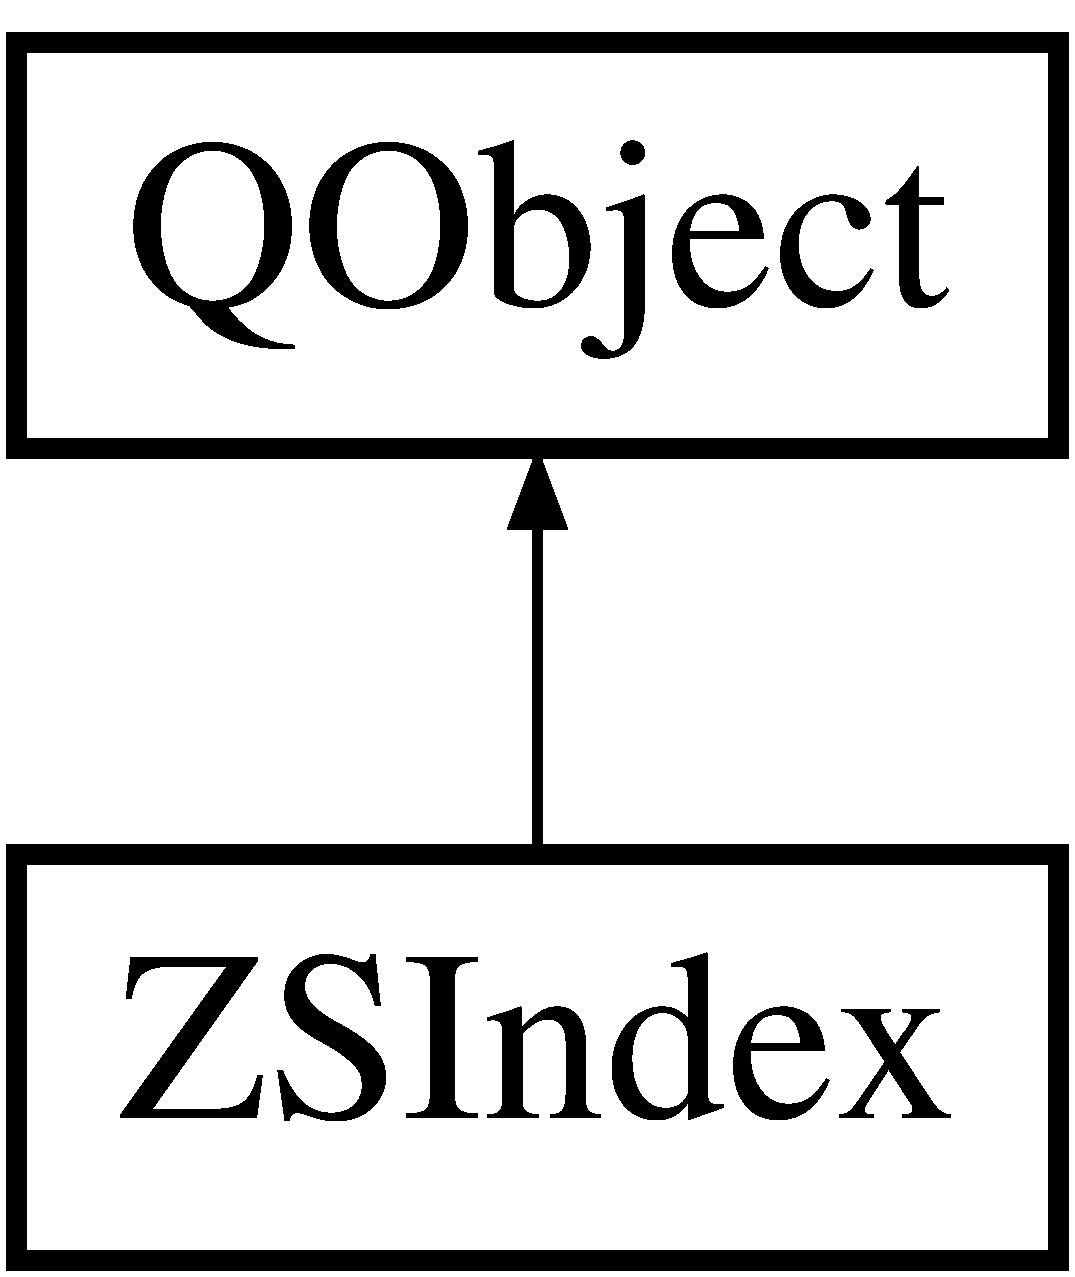
\includegraphics[height=2.000000cm]{class_z_s_index}
\end{center}
\end{figure}
\subsection*{Public Slots}
\begin{DoxyCompactItemize}
\item 
void \hyperlink{class_z_s_index_a709742851eceb8cfc745a0e58d98ee99}{slot\-Update\-Index} ()
\end{DoxyCompactItemize}
\subsection*{Public Member Functions}
\begin{DoxyCompactItemize}
\item 
\hyperlink{class_z_s_index_acae53868cf7e6d16e2f005091d6ffcfe}{Z\-S\-Index} (Q\-Object $\ast$parent=0, \hyperlink{class_z_s_database}{Z\-S\-Database} $\ast$zsdatabase=0)
\item 
void \hyperlink{class_z_s_index_ad18e3601ac62ed2140635ac19ca43b8c}{increase\-Latest\-State} ()
\end{DoxyCompactItemize}


\subsection{Constructor \& Destructor Documentation}
\hypertarget{class_z_s_index_acae53868cf7e6d16e2f005091d6ffcfe}{\index{Z\-S\-Index@{Z\-S\-Index}!Z\-S\-Index@{Z\-S\-Index}}
\index{Z\-S\-Index@{Z\-S\-Index}!ZSIndex@{Z\-S\-Index}}
\subsubsection[{Z\-S\-Index}]{\setlength{\rightskip}{0pt plus 5cm}Z\-S\-Index\-::\-Z\-S\-Index (
\begin{DoxyParamCaption}
\item[{Q\-Object $\ast$}]{parent = {\ttfamily 0}, }
\item[{{\bf Z\-S\-Database} $\ast$}]{zsdatabase = {\ttfamily 0}}
\end{DoxyParamCaption}
)\hspace{0.3cm}{\ttfamily [explicit]}}}\label{class_z_s_index_acae53868cf7e6d16e2f005091d6ffcfe}


\subsection{Member Function Documentation}
\hypertarget{class_z_s_index_ad18e3601ac62ed2140635ac19ca43b8c}{\index{Z\-S\-Index@{Z\-S\-Index}!increase\-Latest\-State@{increase\-Latest\-State}}
\index{increase\-Latest\-State@{increase\-Latest\-State}!ZSIndex@{Z\-S\-Index}}
\subsubsection[{increase\-Latest\-State}]{\setlength{\rightskip}{0pt plus 5cm}void Z\-S\-Index\-::increase\-Latest\-State (
\begin{DoxyParamCaption}
{}
\end{DoxyParamCaption}
)}}\label{class_z_s_index_ad18e3601ac62ed2140635ac19ca43b8c}
\hypertarget{class_z_s_index_a709742851eceb8cfc745a0e58d98ee99}{\index{Z\-S\-Index@{Z\-S\-Index}!slot\-Update\-Index@{slot\-Update\-Index}}
\index{slot\-Update\-Index@{slot\-Update\-Index}!ZSIndex@{Z\-S\-Index}}
\subsubsection[{slot\-Update\-Index}]{\setlength{\rightskip}{0pt plus 5cm}void Z\-S\-Index\-::slot\-Update\-Index (
\begin{DoxyParamCaption}
{}
\end{DoxyParamCaption}
)\hspace{0.3cm}{\ttfamily [slot]}}}\label{class_z_s_index_a709742851eceb8cfc745a0e58d98ee99}


The documentation for this class was generated from the following files\-:\begin{DoxyCompactItemize}
\item 
C\-:/\-Users/\-Tommy/workspace/cpp/zerodesk/\-Zero\-Sync\-Desktop/\hyperlink{zsindex_8h}{zsindex.\-h}\item 
C\-:/\-Users/\-Tommy/workspace/cpp/zerodesk/\-Zero\-Sync\-Desktop/\hyperlink{zsindex_8cpp}{zsindex.\-cpp}\end{DoxyCompactItemize}

\hypertarget{class_z_s_settings}{\section{Z\-S\-Settings Class Reference}
\label{class_z_s_settings}\index{Z\-S\-Settings@{Z\-S\-Settings}}
}


{\ttfamily \#include $<$zssettings.\-h$>$}

Inheritance diagram for Z\-S\-Settings\-:\begin{figure}[H]
\begin{center}
\leavevmode
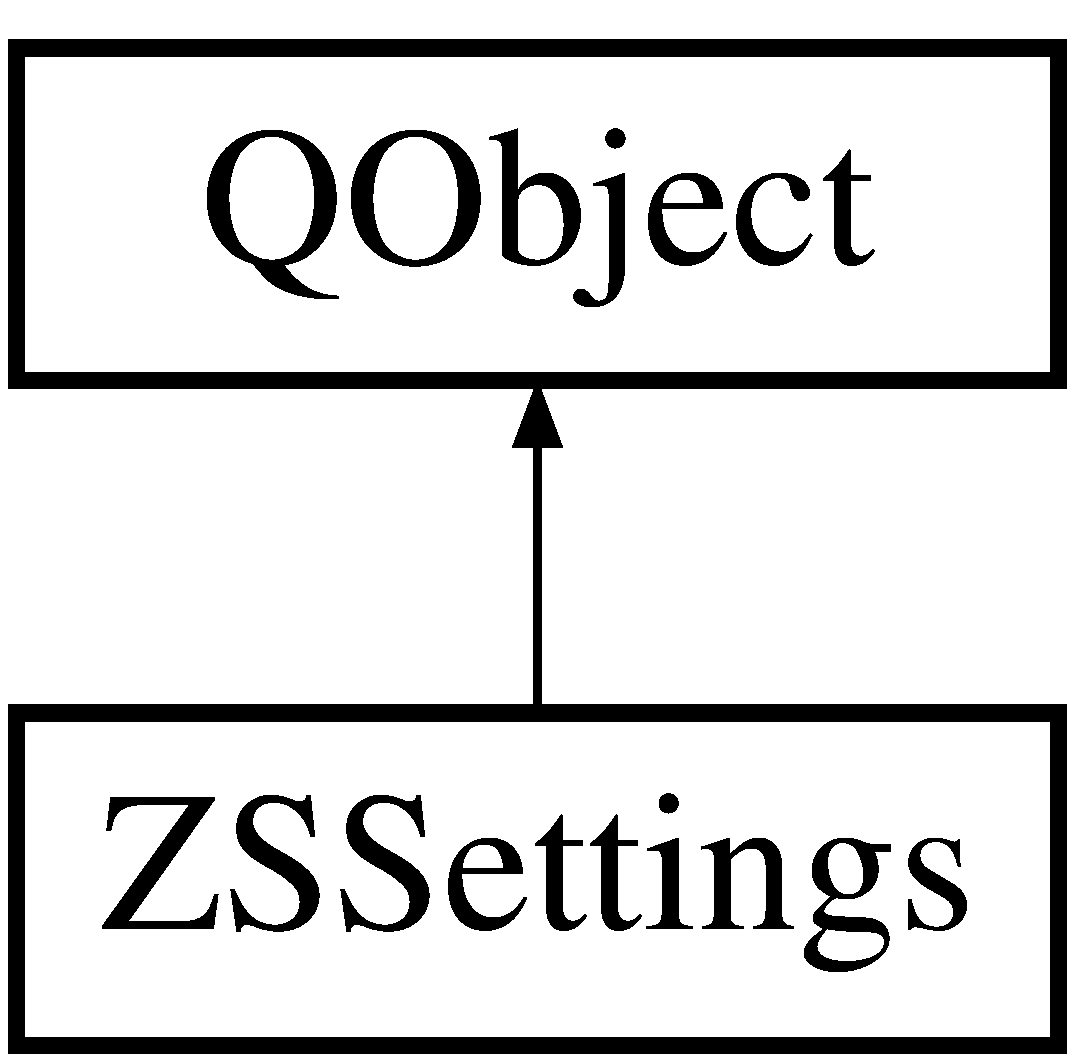
\includegraphics[height=2.000000cm]{class_z_s_settings}
\end{center}
\end{figure}
\subsection*{Public Member Functions}
\begin{DoxyCompactItemize}
\item 
\hyperlink{class_z_s_settings_a03b2e67c7c6b0360be693761c34d7fe1}{Z\-S\-Settings} (Q\-Object $\ast$parent=0)
\item 
bool \hyperlink{class_z_s_settings_adb668cc8ff7cb7a06a00614ba88747c0}{exist\-Settings} ()
\item 
void \hyperlink{class_z_s_settings_adaae344d9e45743c89ff6e8df3ca5839}{set\-Zero\-Sync\-Directory} (Q\-String)
\item 
void \hyperlink{class_z_s_settings_abdb80b46c5a5310cabab0337e74f9a8b}{set\-Sync\-Interval} (int)
\item 
Q\-String \hyperlink{class_z_s_settings_a449de5e3a46a864f0e507d653ebee9db}{get\-Zero\-Sync\-Directory} ()
\item 
int \hyperlink{class_z_s_settings_a6b645f032aaef3f62b67c4471794703e}{get\-Sync\-Interval} ()
\end{DoxyCompactItemize}


\subsection{Constructor \& Destructor Documentation}
\hypertarget{class_z_s_settings_a03b2e67c7c6b0360be693761c34d7fe1}{\index{Z\-S\-Settings@{Z\-S\-Settings}!Z\-S\-Settings@{Z\-S\-Settings}}
\index{Z\-S\-Settings@{Z\-S\-Settings}!ZSSettings@{Z\-S\-Settings}}
\subsubsection[{Z\-S\-Settings}]{\setlength{\rightskip}{0pt plus 5cm}Z\-S\-Settings\-::\-Z\-S\-Settings (
\begin{DoxyParamCaption}
\item[{Q\-Object $\ast$}]{parent = {\ttfamily 0}}
\end{DoxyParamCaption}
)\hspace{0.3cm}{\ttfamily [explicit]}}}\label{class_z_s_settings_a03b2e67c7c6b0360be693761c34d7fe1}


\subsection{Member Function Documentation}
\hypertarget{class_z_s_settings_adb668cc8ff7cb7a06a00614ba88747c0}{\index{Z\-S\-Settings@{Z\-S\-Settings}!exist\-Settings@{exist\-Settings}}
\index{exist\-Settings@{exist\-Settings}!ZSSettings@{Z\-S\-Settings}}
\subsubsection[{exist\-Settings}]{\setlength{\rightskip}{0pt plus 5cm}bool Z\-S\-Settings\-::exist\-Settings (
\begin{DoxyParamCaption}
{}
\end{DoxyParamCaption}
)}}\label{class_z_s_settings_adb668cc8ff7cb7a06a00614ba88747c0}
\hypertarget{class_z_s_settings_a6b645f032aaef3f62b67c4471794703e}{\index{Z\-S\-Settings@{Z\-S\-Settings}!get\-Sync\-Interval@{get\-Sync\-Interval}}
\index{get\-Sync\-Interval@{get\-Sync\-Interval}!ZSSettings@{Z\-S\-Settings}}
\subsubsection[{get\-Sync\-Interval}]{\setlength{\rightskip}{0pt plus 5cm}int Z\-S\-Settings\-::get\-Sync\-Interval (
\begin{DoxyParamCaption}
{}
\end{DoxyParamCaption}
)}}\label{class_z_s_settings_a6b645f032aaef3f62b67c4471794703e}
\hypertarget{class_z_s_settings_a449de5e3a46a864f0e507d653ebee9db}{\index{Z\-S\-Settings@{Z\-S\-Settings}!get\-Zero\-Sync\-Directory@{get\-Zero\-Sync\-Directory}}
\index{get\-Zero\-Sync\-Directory@{get\-Zero\-Sync\-Directory}!ZSSettings@{Z\-S\-Settings}}
\subsubsection[{get\-Zero\-Sync\-Directory}]{\setlength{\rightskip}{0pt plus 5cm}Q\-String Z\-S\-Settings\-::get\-Zero\-Sync\-Directory (
\begin{DoxyParamCaption}
{}
\end{DoxyParamCaption}
)}}\label{class_z_s_settings_a449de5e3a46a864f0e507d653ebee9db}
\hypertarget{class_z_s_settings_abdb80b46c5a5310cabab0337e74f9a8b}{\index{Z\-S\-Settings@{Z\-S\-Settings}!set\-Sync\-Interval@{set\-Sync\-Interval}}
\index{set\-Sync\-Interval@{set\-Sync\-Interval}!ZSSettings@{Z\-S\-Settings}}
\subsubsection[{set\-Sync\-Interval}]{\setlength{\rightskip}{0pt plus 5cm}void Z\-S\-Settings\-::set\-Sync\-Interval (
\begin{DoxyParamCaption}
\item[{int}]{seconds}
\end{DoxyParamCaption}
)}}\label{class_z_s_settings_abdb80b46c5a5310cabab0337e74f9a8b}
\hypertarget{class_z_s_settings_adaae344d9e45743c89ff6e8df3ca5839}{\index{Z\-S\-Settings@{Z\-S\-Settings}!set\-Zero\-Sync\-Directory@{set\-Zero\-Sync\-Directory}}
\index{set\-Zero\-Sync\-Directory@{set\-Zero\-Sync\-Directory}!ZSSettings@{Z\-S\-Settings}}
\subsubsection[{set\-Zero\-Sync\-Directory}]{\setlength{\rightskip}{0pt plus 5cm}void Z\-S\-Settings\-::set\-Zero\-Sync\-Directory (
\begin{DoxyParamCaption}
\item[{Q\-String}]{path}
\end{DoxyParamCaption}
)}}\label{class_z_s_settings_adaae344d9e45743c89ff6e8df3ca5839}


The documentation for this class was generated from the following files\-:\begin{DoxyCompactItemize}
\item 
C\-:/\-Users/\-Tommy/workspace/cpp/zerodesk/\-Zero\-Sync\-Desktop/\hyperlink{zssettings_8h}{zssettings.\-h}\item 
C\-:/\-Users/\-Tommy/workspace/cpp/zerodesk/\-Zero\-Sync\-Desktop/\hyperlink{zssettings_8cpp}{zssettings.\-cpp}\end{DoxyCompactItemize}

\hypertarget{class_z_s_setup_wizard}{\section{Z\-S\-Setup\-Wizard Class Reference}
\label{class_z_s_setup_wizard}\index{Z\-S\-Setup\-Wizard@{Z\-S\-Setup\-Wizard}}
}


{\ttfamily \#include $<$zssetupwizard.\-h$>$}

Inheritance diagram for Z\-S\-Setup\-Wizard\-:\begin{figure}[H]
\begin{center}
\leavevmode
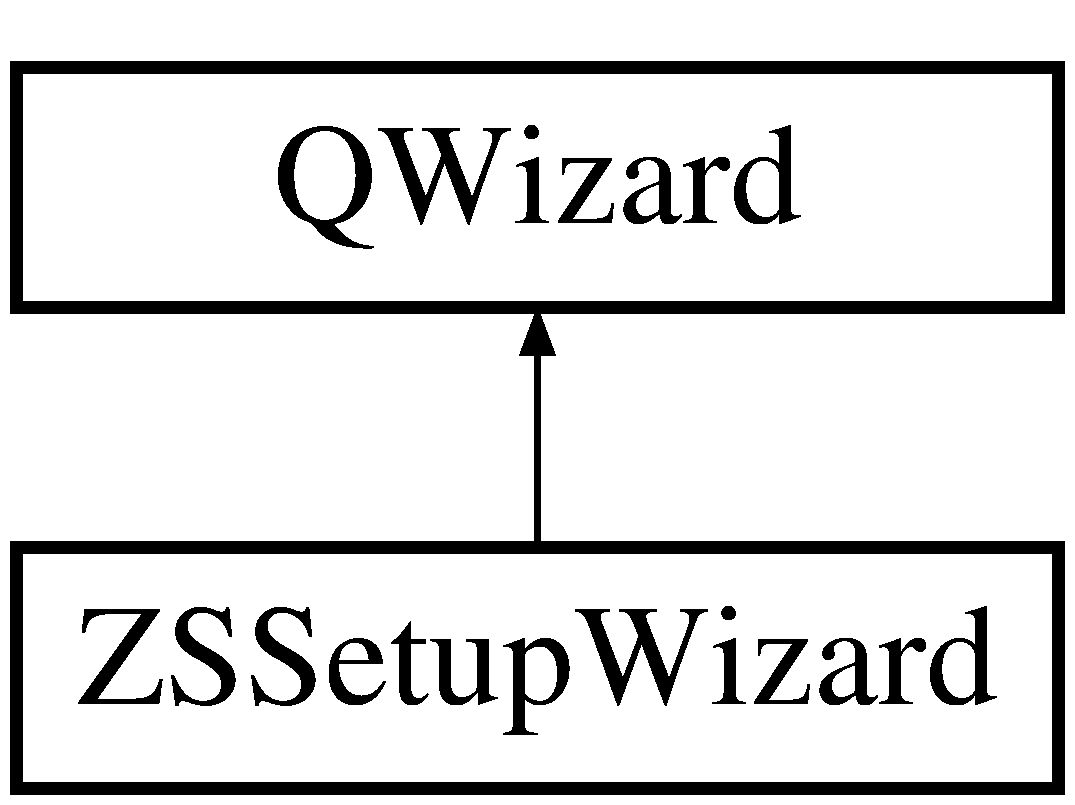
\includegraphics[height=2.000000cm]{class_z_s_setup_wizard}
\end{center}
\end{figure}
\subsection*{Public Member Functions}
\begin{DoxyCompactItemize}
\item 
\hyperlink{class_z_s_setup_wizard_a7e2200c20b64930253001adaf6d51a7d}{Z\-S\-Setup\-Wizard} (Q\-Object $\ast$parent=0)
\end{DoxyCompactItemize}


\subsection{Constructor \& Destructor Documentation}
\hypertarget{class_z_s_setup_wizard_a7e2200c20b64930253001adaf6d51a7d}{\index{Z\-S\-Setup\-Wizard@{Z\-S\-Setup\-Wizard}!Z\-S\-Setup\-Wizard@{Z\-S\-Setup\-Wizard}}
\index{Z\-S\-Setup\-Wizard@{Z\-S\-Setup\-Wizard}!ZSSetupWizard@{Z\-S\-Setup\-Wizard}}
\subsubsection[{Z\-S\-Setup\-Wizard}]{\setlength{\rightskip}{0pt plus 5cm}Z\-S\-Setup\-Wizard\-::\-Z\-S\-Setup\-Wizard (
\begin{DoxyParamCaption}
\item[{Q\-Object $\ast$}]{parent = {\ttfamily 0}}
\end{DoxyParamCaption}
)\hspace{0.3cm}{\ttfamily [explicit]}}}\label{class_z_s_setup_wizard_a7e2200c20b64930253001adaf6d51a7d}


The documentation for this class was generated from the following files\-:\begin{DoxyCompactItemize}
\item 
C\-:/\-Users/adorno/github/zerodesk/\-Zero\-Sync\-Desktop/\hyperlink{zssetupwizard_8h}{zssetupwizard.\-h}\item 
C\-:/\-Users/adorno/github/zerodesk/\-Zero\-Sync\-Desktop/\hyperlink{zssetupwizard_8cpp}{zssetupwizard.\-cpp}\end{DoxyCompactItemize}

\input{class_z_s_sync_wizard_page}
\chapter{File Documentation}
\hypertarget{main_8cpp}{\section{C\-:/\-Users/\-Tommy/workspace/cpp/zerodesk/\-Zero\-Sync\-Desktop/main.cpp File Reference}
\label{main_8cpp}\index{C\-:/\-Users/\-Tommy/workspace/cpp/zerodesk/\-Zero\-Sync\-Desktop/main.\-cpp@{C\-:/\-Users/\-Tommy/workspace/cpp/zerodesk/\-Zero\-Sync\-Desktop/main.\-cpp}}
}
{\ttfamily \#include \char`\"{}mainwindow.\-h\char`\"{}}\\*
{\ttfamily \#include $<$Q\-Application$>$}\\*
{\ttfamily \#include $<$Q\-Shared\-Memory$>$}\\*
\subsection*{Functions}
\begin{DoxyCompactItemize}
\item 
int \hyperlink{main_8cpp_a0ddf1224851353fc92bfbff6f499fa97}{main} (int argc, char $\ast$argv\mbox{[}$\,$\mbox{]})
\end{DoxyCompactItemize}


\subsection{Function Documentation}
\hypertarget{main_8cpp_a0ddf1224851353fc92bfbff6f499fa97}{\index{main.\-cpp@{main.\-cpp}!main@{main}}
\index{main@{main}!main.cpp@{main.\-cpp}}
\subsubsection[{main}]{\setlength{\rightskip}{0pt plus 5cm}int main (
\begin{DoxyParamCaption}
\item[{int}]{argc, }
\item[{char $\ast$}]{argv\mbox{[}$\,$\mbox{]}}
\end{DoxyParamCaption}
)}}\label{main_8cpp_a0ddf1224851353fc92bfbff6f499fa97}

\hypertarget{mainwindow_8cpp}{\section{C\-:/\-Users/\-Tommy/workspace/cpp/zerodesk/\-Zero\-Sync\-Desktop/mainwindow.cpp File Reference}
\label{mainwindow_8cpp}\index{C\-:/\-Users/\-Tommy/workspace/cpp/zerodesk/\-Zero\-Sync\-Desktop/mainwindow.\-cpp@{C\-:/\-Users/\-Tommy/workspace/cpp/zerodesk/\-Zero\-Sync\-Desktop/mainwindow.\-cpp}}
}
{\ttfamily \#include \char`\"{}mainwindow.\-h\char`\"{}}\\*
{\ttfamily \#include \char`\"{}ui\-\_\-mainwindow.\-h\char`\"{}}\\*

\hypertarget{mainwindow_8h}{\section{C\-:/\-Users/\-Tommy/workspace/cpp/zerodesk/\-Zero\-Sync\-Desktop/mainwindow.h File Reference}
\label{mainwindow_8h}\index{C\-:/\-Users/\-Tommy/workspace/cpp/zerodesk/\-Zero\-Sync\-Desktop/mainwindow.\-h@{C\-:/\-Users/\-Tommy/workspace/cpp/zerodesk/\-Zero\-Sync\-Desktop/mainwindow.\-h}}
}
{\ttfamily \#include $<$Q\-Main\-Window$>$}\\*
{\ttfamily \#include $<$Q\-System\-Tray\-Icon$>$}\\*
{\ttfamily \#include $<$Q\-Menu$>$}\\*
{\ttfamily \#include $<$Q\-Close\-Event$>$}\\*
{\ttfamily \#include $<$iostream$>$}\\*
{\ttfamily \#include $<$Q\-File\-Dialog$>$}\\*
{\ttfamily \#include $<$Qt\-Debug$>$}\\*
{\ttfamily \#include $<$Q\-Message\-Box$>$}\\*
{\ttfamily \#include $<$Q\-Timer$>$}\\*
{\ttfamily \#include $<$Q\-Button\-Group$>$}\\*
{\ttfamily \#include \char`\"{}zsfilesystemwatcher.\-h\char`\"{}}\\*
{\ttfamily \#include \char`\"{}zsdatabase.\-h\char`\"{}}\\*
{\ttfamily \#include \char`\"{}zsindex.\-h\char`\"{}}\\*
{\ttfamily \#include \char`\"{}zssetupwizard.\-h\char`\"{}}\\*
{\ttfamily \#include \char`\"{}zssettings.\-h\char`\"{}}\\*
\subsection*{Classes}
\begin{DoxyCompactItemize}
\item 
class \hyperlink{class_main_window}{Main\-Window}
\end{DoxyCompactItemize}
\subsection*{Namespaces}
\begin{DoxyCompactItemize}
\item 
\hyperlink{namespace_ui}{Ui}
\end{DoxyCompactItemize}

\hypertarget{zsdatabase_8cpp}{\section{C\-:/\-Users/adorno/github/zerodesk/\-Zero\-Sync\-Desktop/zsdatabase.cpp File Reference}
\label{zsdatabase_8cpp}\index{C\-:/\-Users/adorno/github/zerodesk/\-Zero\-Sync\-Desktop/zsdatabase.\-cpp@{C\-:/\-Users/adorno/github/zerodesk/\-Zero\-Sync\-Desktop/zsdatabase.\-cpp}}
}
{\ttfamily \#include \char`\"{}zsdatabase.\-h\char`\"{}}\\*

\hypertarget{zsdatabase_8h}{\section{C\-:/\-Users/adorno/github/zerodesk/\-Zero\-Sync\-Desktop/zsdatabase.h File Reference}
\label{zsdatabase_8h}\index{C\-:/\-Users/adorno/github/zerodesk/\-Zero\-Sync\-Desktop/zsdatabase.\-h@{C\-:/\-Users/adorno/github/zerodesk/\-Zero\-Sync\-Desktop/zsdatabase.\-h}}
}
{\ttfamily \#include $<$Q\-Object$>$}\\*
{\ttfamily \#include $<$Q\-Sql\-Database$>$}\\*
{\ttfamily \#include $<$Q\-Standard\-Paths$>$}\\*
{\ttfamily \#include $<$Q\-File$>$}\\*
{\ttfamily \#include $<$Q\-Sql\-Query$>$}\\*
{\ttfamily \#include $<$Q\-Text\-Stream$>$}\\*
{\ttfamily \#include $<$Qt\-Debug$>$}\\*
\subsection*{Classes}
\begin{DoxyCompactItemize}
\item 
class \hyperlink{class_z_s_database}{Z\-S\-Database}
\end{DoxyCompactItemize}

\input{zsdirectorywizardpage_8cpp}
\input{zsdirectorywizardpage_8h}
\hypertarget{zsfilemetadata_8cpp}{\section{C\-:/\-Users/adorno/github/zerodesk/\-Zero\-Sync\-Desktop/zsfilemetadata.cpp File Reference}
\label{zsfilemetadata_8cpp}\index{C\-:/\-Users/adorno/github/zerodesk/\-Zero\-Sync\-Desktop/zsfilemetadata.\-cpp@{C\-:/\-Users/adorno/github/zerodesk/\-Zero\-Sync\-Desktop/zsfilemetadata.\-cpp}}
}
{\ttfamily \#include \char`\"{}zsfilemetadata.\-h\char`\"{}}\\*

\hypertarget{zsfilemetadata_8h}{\section{C\-:/\-Users/\-Tommy/workspace/cpp/zerodesk/\-Zero\-Sync\-Desktop/zsfilemetadata.h File Reference}
\label{zsfilemetadata_8h}\index{C\-:/\-Users/\-Tommy/workspace/cpp/zerodesk/\-Zero\-Sync\-Desktop/zsfilemetadata.\-h@{C\-:/\-Users/\-Tommy/workspace/cpp/zerodesk/\-Zero\-Sync\-Desktop/zsfilemetadata.\-h}}
}
{\ttfamily \#include $<$Q\-Object$>$}\\*
{\ttfamily \#include $<$Qt\-Debug$>$}\\*
{\ttfamily \#include $<$Q\-File\-Info$>$}\\*
{\ttfamily \#include $<$Q\-Cryptographic\-Hash$>$}\\*
{\ttfamily \#include $<$Q\-File$>$}\\*
{\ttfamily \#include $<$Q\-Byte\-Array$>$}\\*
{\ttfamily \#include $<$Q\-Date\-Time$>$}\\*
\subsection*{Classes}
\begin{DoxyCompactItemize}
\item 
class \hyperlink{class_z_s_file_meta_data}{Z\-S\-File\-Meta\-Data}
\end{DoxyCompactItemize}

\hypertarget{zsfilesystemwatcher_8cpp}{\section{C\-:/\-Users/adorno/github/zerodesk/\-Zero\-Sync\-Desktop/zsfilesystemwatcher.cpp File Reference}
\label{zsfilesystemwatcher_8cpp}\index{C\-:/\-Users/adorno/github/zerodesk/\-Zero\-Sync\-Desktop/zsfilesystemwatcher.\-cpp@{C\-:/\-Users/adorno/github/zerodesk/\-Zero\-Sync\-Desktop/zsfilesystemwatcher.\-cpp}}
}
{\ttfamily \#include \char`\"{}zsfilesystemwatcher.\-h\char`\"{}}\\*

\hypertarget{zsfilesystemwatcher_8h}{\section{C\-:/\-Users/adorno/github/zerodesk/\-Zero\-Sync\-Desktop/zsfilesystemwatcher.h File Reference}
\label{zsfilesystemwatcher_8h}\index{C\-:/\-Users/adorno/github/zerodesk/\-Zero\-Sync\-Desktop/zsfilesystemwatcher.\-h@{C\-:/\-Users/adorno/github/zerodesk/\-Zero\-Sync\-Desktop/zsfilesystemwatcher.\-h}}
}
{\ttfamily \#include $<$Q\-Object$>$}\\*
{\ttfamily \#include $<$Q\-File\-System\-Watcher$>$}\\*
{\ttfamily \#include $<$Q\-Dir$>$}\\*
{\ttfamily \#include $<$Qt\-Debug$>$}\\*
{\ttfamily \#include $<$Q\-Dir\-Iterator$>$}\\*
{\ttfamily \#include $<$Q\-Cryptographic\-Hash$>$}\\*
{\ttfamily \#include $<$Q\-Date\-Time$>$}\\*
{\ttfamily \#include $<$Q\-Standard\-Paths$>$}\\*
{\ttfamily \#include \char`\"{}zsdatabase.\-h\char`\"{}}\\*
{\ttfamily \#include \char`\"{}zsfilemetadata.\-h\char`\"{}}\\*
{\ttfamily \#include \char`\"{}zsindex.\-h\char`\"{}}\\*
\subsection*{Classes}
\begin{DoxyCompactItemize}
\item 
class \hyperlink{class_z_s_file_system_watcher}{Z\-S\-File\-System\-Watcher}
\end{DoxyCompactItemize}

\hypertarget{zsindex_8cpp}{\section{C\-:/\-Users/\-Tommy/workspace/cpp/zerodesk/\-Zero\-Sync\-Desktop/zsindex.cpp File Reference}
\label{zsindex_8cpp}\index{C\-:/\-Users/\-Tommy/workspace/cpp/zerodesk/\-Zero\-Sync\-Desktop/zsindex.\-cpp@{C\-:/\-Users/\-Tommy/workspace/cpp/zerodesk/\-Zero\-Sync\-Desktop/zsindex.\-cpp}}
}
{\ttfamily \#include \char`\"{}zsindex.\-h\char`\"{}}\\*

\hypertarget{zsindex_8h}{\section{C\-:/\-Users/\-Tommy/workspace/cpp/zerodesk/\-Zero\-Sync\-Desktop/zsindex.h File Reference}
\label{zsindex_8h}\index{C\-:/\-Users/\-Tommy/workspace/cpp/zerodesk/\-Zero\-Sync\-Desktop/zsindex.\-h@{C\-:/\-Users/\-Tommy/workspace/cpp/zerodesk/\-Zero\-Sync\-Desktop/zsindex.\-h}}
}
{\ttfamily \#include $<$Q\-Object$>$}\\*
{\ttfamily \#include $<$Qt\-Debug$>$}\\*
{\ttfamily \#include $<$Q\-Sql\-Query$>$}\\*
{\ttfamily \#include $<$Q\-Sql\-Database$>$}\\*
{\ttfamily \#include \char`\"{}zsdatabase.\-h\char`\"{}}\\*
{\ttfamily \#include \char`\"{}zsfilemetadata.\-h\char`\"{}}\\*
\subsection*{Classes}
\begin{DoxyCompactItemize}
\item 
class \hyperlink{class_z_s_index}{Z\-S\-Index}
\end{DoxyCompactItemize}

\hypertarget{zssettings_8cpp}{\section{C\-:/\-Users/adorno/github/zerodesk/\-Zero\-Sync\-Desktop/zssettings.cpp File Reference}
\label{zssettings_8cpp}\index{C\-:/\-Users/adorno/github/zerodesk/\-Zero\-Sync\-Desktop/zssettings.\-cpp@{C\-:/\-Users/adorno/github/zerodesk/\-Zero\-Sync\-Desktop/zssettings.\-cpp}}
}
{\ttfamily \#include \char`\"{}zssettings.\-h\char`\"{}}\\*

\hypertarget{zssettings_8h}{\section{C\-:/\-Users/\-Tommy/workspace/cpp/zerodesk/\-Zero\-Sync\-Desktop/zssettings.h File Reference}
\label{zssettings_8h}\index{C\-:/\-Users/\-Tommy/workspace/cpp/zerodesk/\-Zero\-Sync\-Desktop/zssettings.\-h@{C\-:/\-Users/\-Tommy/workspace/cpp/zerodesk/\-Zero\-Sync\-Desktop/zssettings.\-h}}
}
{\ttfamily \#include $<$Q\-Object$>$}\\*
{\ttfamily \#include $<$Q\-Settings$>$}\\*
\subsection*{Classes}
\begin{DoxyCompactItemize}
\item 
class \hyperlink{class_z_s_settings}{Z\-S\-Settings}
\end{DoxyCompactItemize}

\hypertarget{zssetupwizard_8cpp}{\section{C\-:/\-Users/adorno/github/zerodesk/\-Zero\-Sync\-Desktop/zssetupwizard.cpp File Reference}
\label{zssetupwizard_8cpp}\index{C\-:/\-Users/adorno/github/zerodesk/\-Zero\-Sync\-Desktop/zssetupwizard.\-cpp@{C\-:/\-Users/adorno/github/zerodesk/\-Zero\-Sync\-Desktop/zssetupwizard.\-cpp}}
}
{\ttfamily \#include \char`\"{}zssetupwizard.\-h\char`\"{}}\\*

\hypertarget{zssetupwizard_8h}{\section{C\-:/\-Users/adorno/github/zerodesk/\-Zero\-Sync\-Desktop/zssetupwizard.h File Reference}
\label{zssetupwizard_8h}\index{C\-:/\-Users/adorno/github/zerodesk/\-Zero\-Sync\-Desktop/zssetupwizard.\-h@{C\-:/\-Users/adorno/github/zerodesk/\-Zero\-Sync\-Desktop/zssetupwizard.\-h}}
}
{\ttfamily \#include $<$Q\-Object$>$}\\*
{\ttfamily \#include $<$Q\-Wizard$>$}\\*
{\ttfamily \#include $<$Q\-Label$>$}\\*
{\ttfamily \#include $<$Q\-V\-Box\-Layout$>$}\\*
{\ttfamily \#include $<$Q\-Line\-Edit$>$}\\*
{\ttfamily \#include $<$Q\-Wizard\-Page$>$}\\*
{\ttfamily \#include $<$Q\-Grid\-Layout$>$}\\*
\subsection*{Classes}
\begin{DoxyCompactItemize}
\item 
class \hyperlink{class_z_s_setup_wizard}{Z\-S\-Setup\-Wizard}
\end{DoxyCompactItemize}

\input{zssyncwizardpage_8cpp}
\input{zssyncwizardpage_8h}
%--- End generated contents ---

% Index
\newpage
\phantomsection
\addcontentsline{toc}{chapter}{Index}
\printindex

\end{document}
